
\section{Methodology}

\subsection{Participants}

The study is conducted on 22 participants. Participants are mainly composed of engineering students. The participant set includes 15 males and 7 females.
The age of participants is between 19 and 22 years old. Exception for three participants that are older than 22 years old. 


\subsection{Procedure}

We introduced the subject telling participants : 
"We're in the very near future. You are looking at plants that make music when you physically interact with them (it is not actually the case, but imagine it). Explore their capabilities."
Using this prompt, we tried not to bridle them to much but approach them to the physical interaction component.
Subsequently, participants were given time to explore the potential musical capacities of the plants at their own pace.
We conducted the study without providing any guidance during the exploration phase.
In instances where participants encountered difficulty initiating exploration, the prompt was reiterated to encourage the participants to explore.
This methodological approach was designed to capture the intuitive and natural human-plant interaction.
Also, we avoided any kind of communication or talking between 2 participants to reduce the potential bias.


\subsection{Materials/Tools}

To proceed and conduct this user study, we chose 3 different plants from 3 different species.

\newpage

\subsubsection{Dracaena}
It has long leaves and fragile perceived trunk but also flexible. The plant is 95 cm tall.

\begin{figure}[ht]
    \centering
    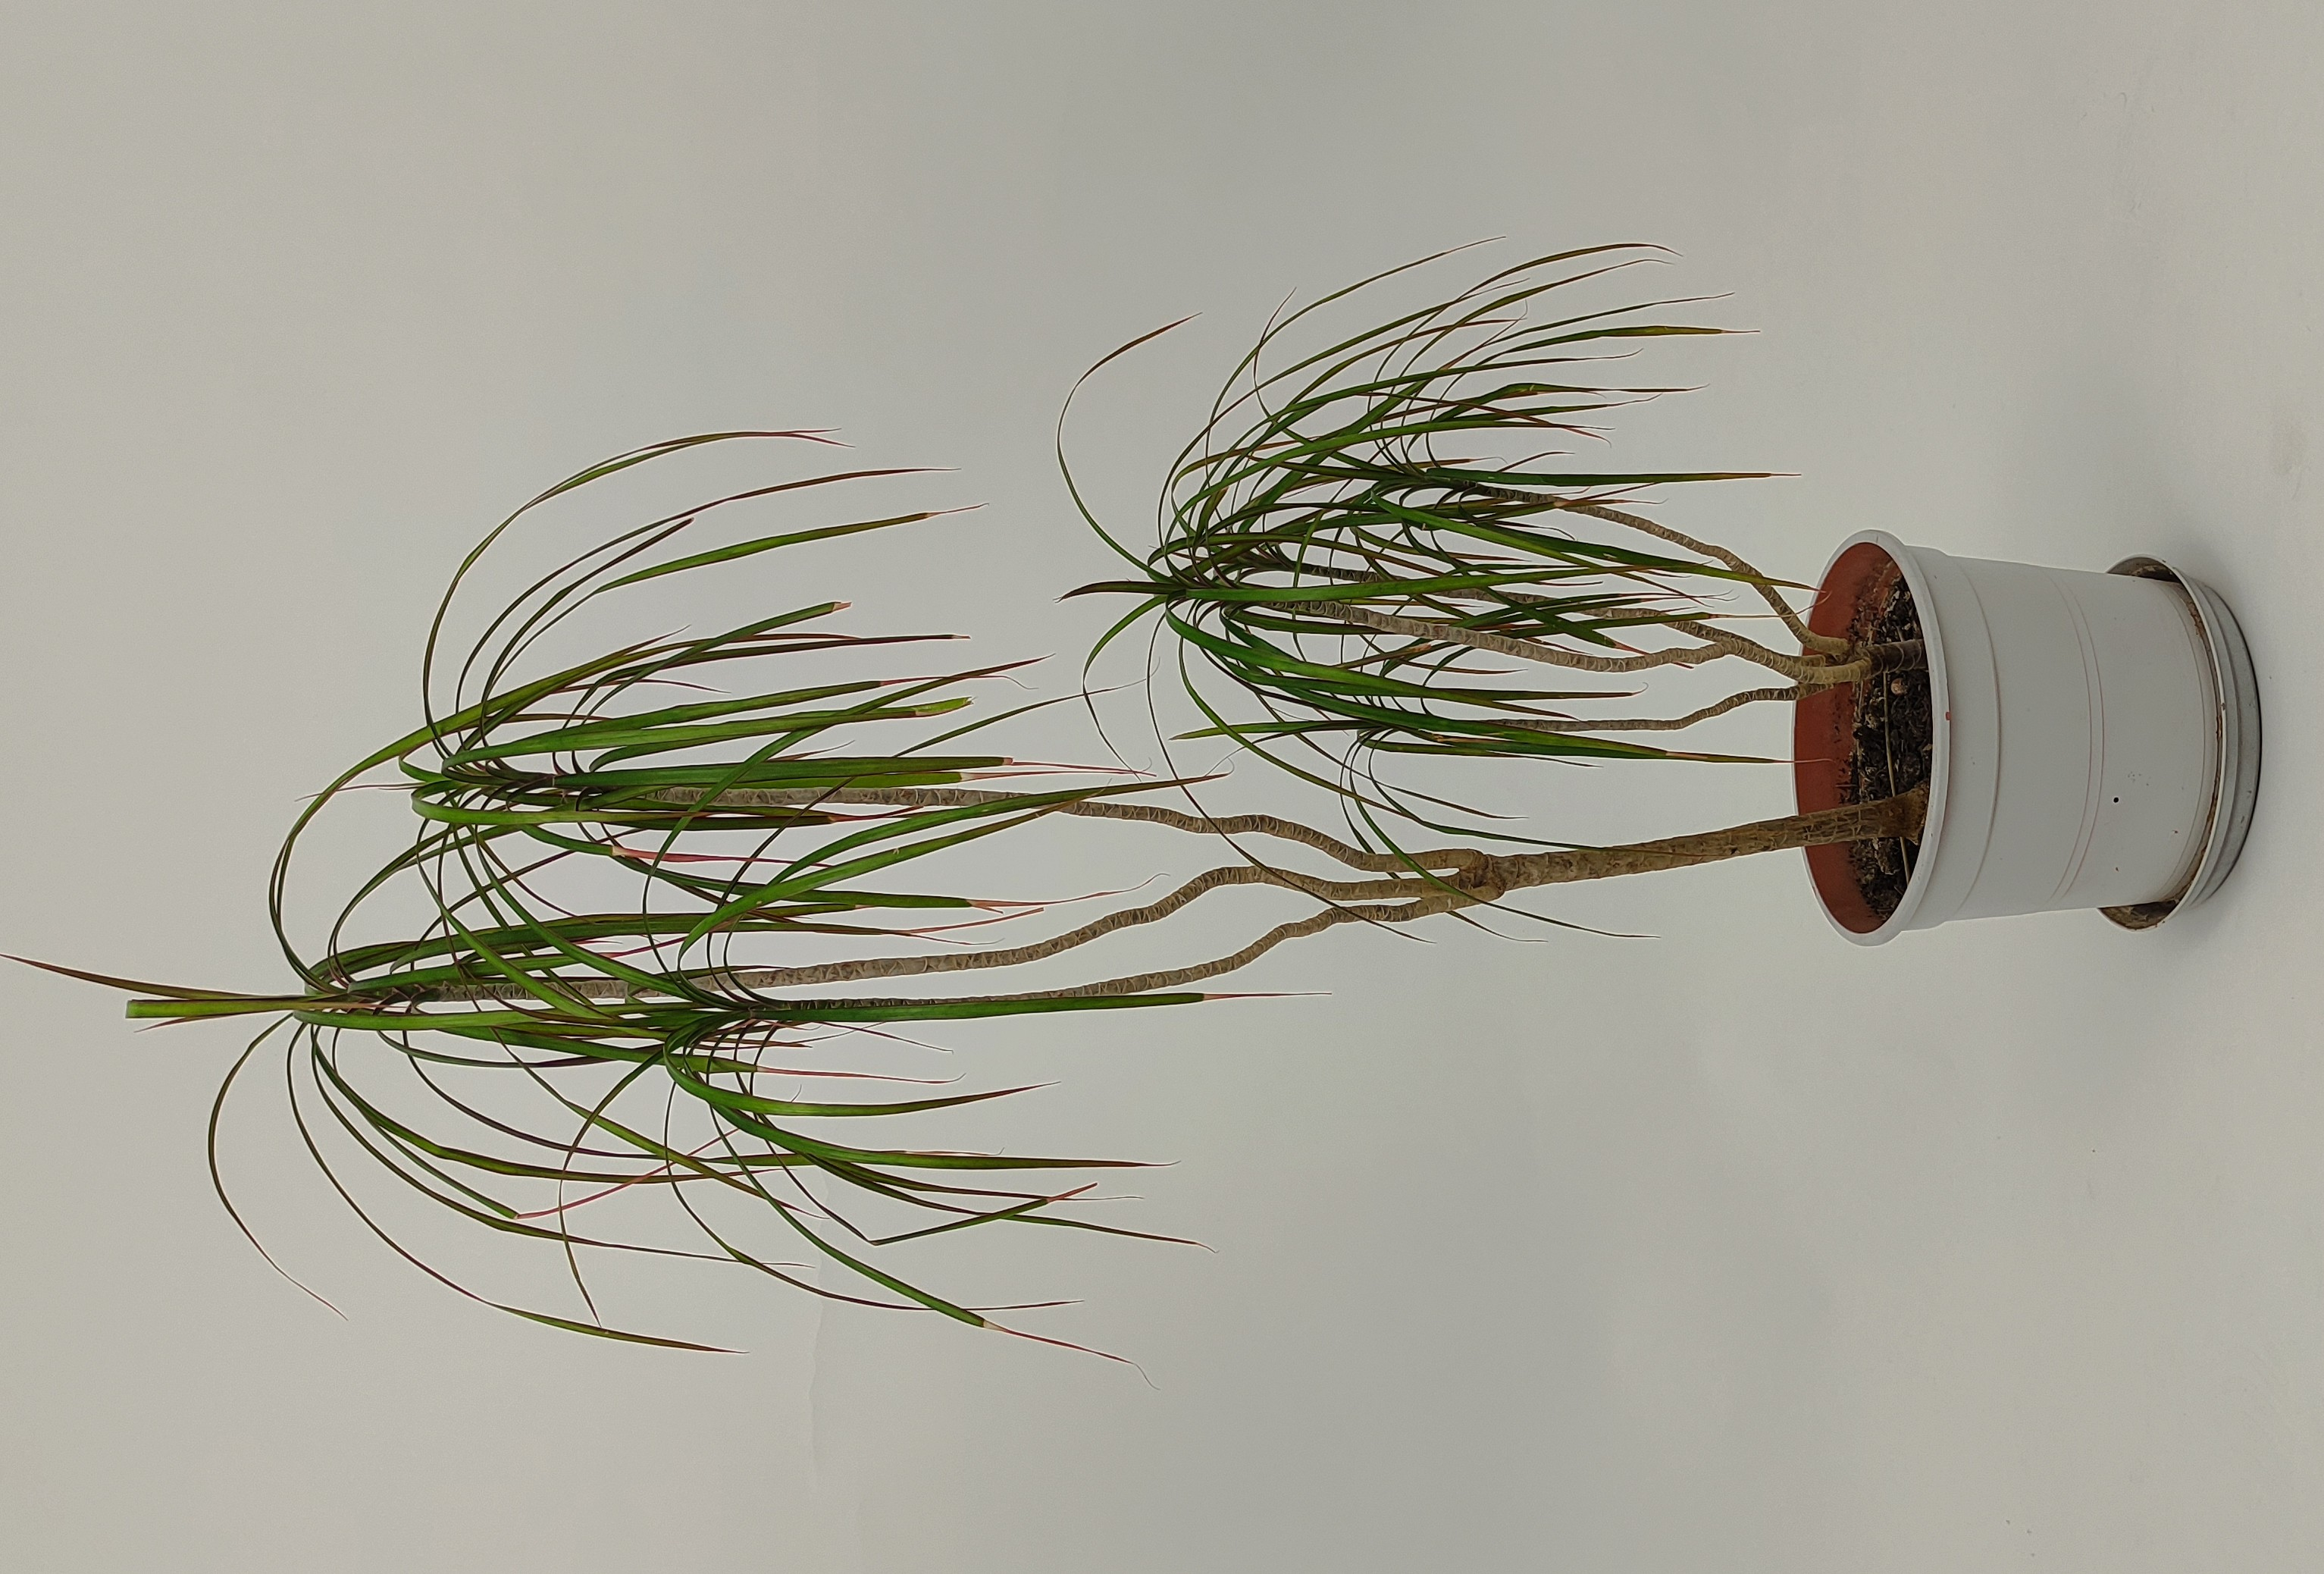
\includegraphics[width=0.42\textwidth, angle=-90]{Images/small_plant.jpg}
    \caption{The plant N°1 is a \textit{Dracaena}.}
    
    \vspace{-0.5cm}
    \label{fig:small_plant}
    \vspace{0.2cm}
\end{figure}




\subsubsection{Pachira glabra}

We chose to use this plant for its large leaves and its wide trunk.
The plant is 110 cm tall.
\begin{figure}[ht]
    \centering
    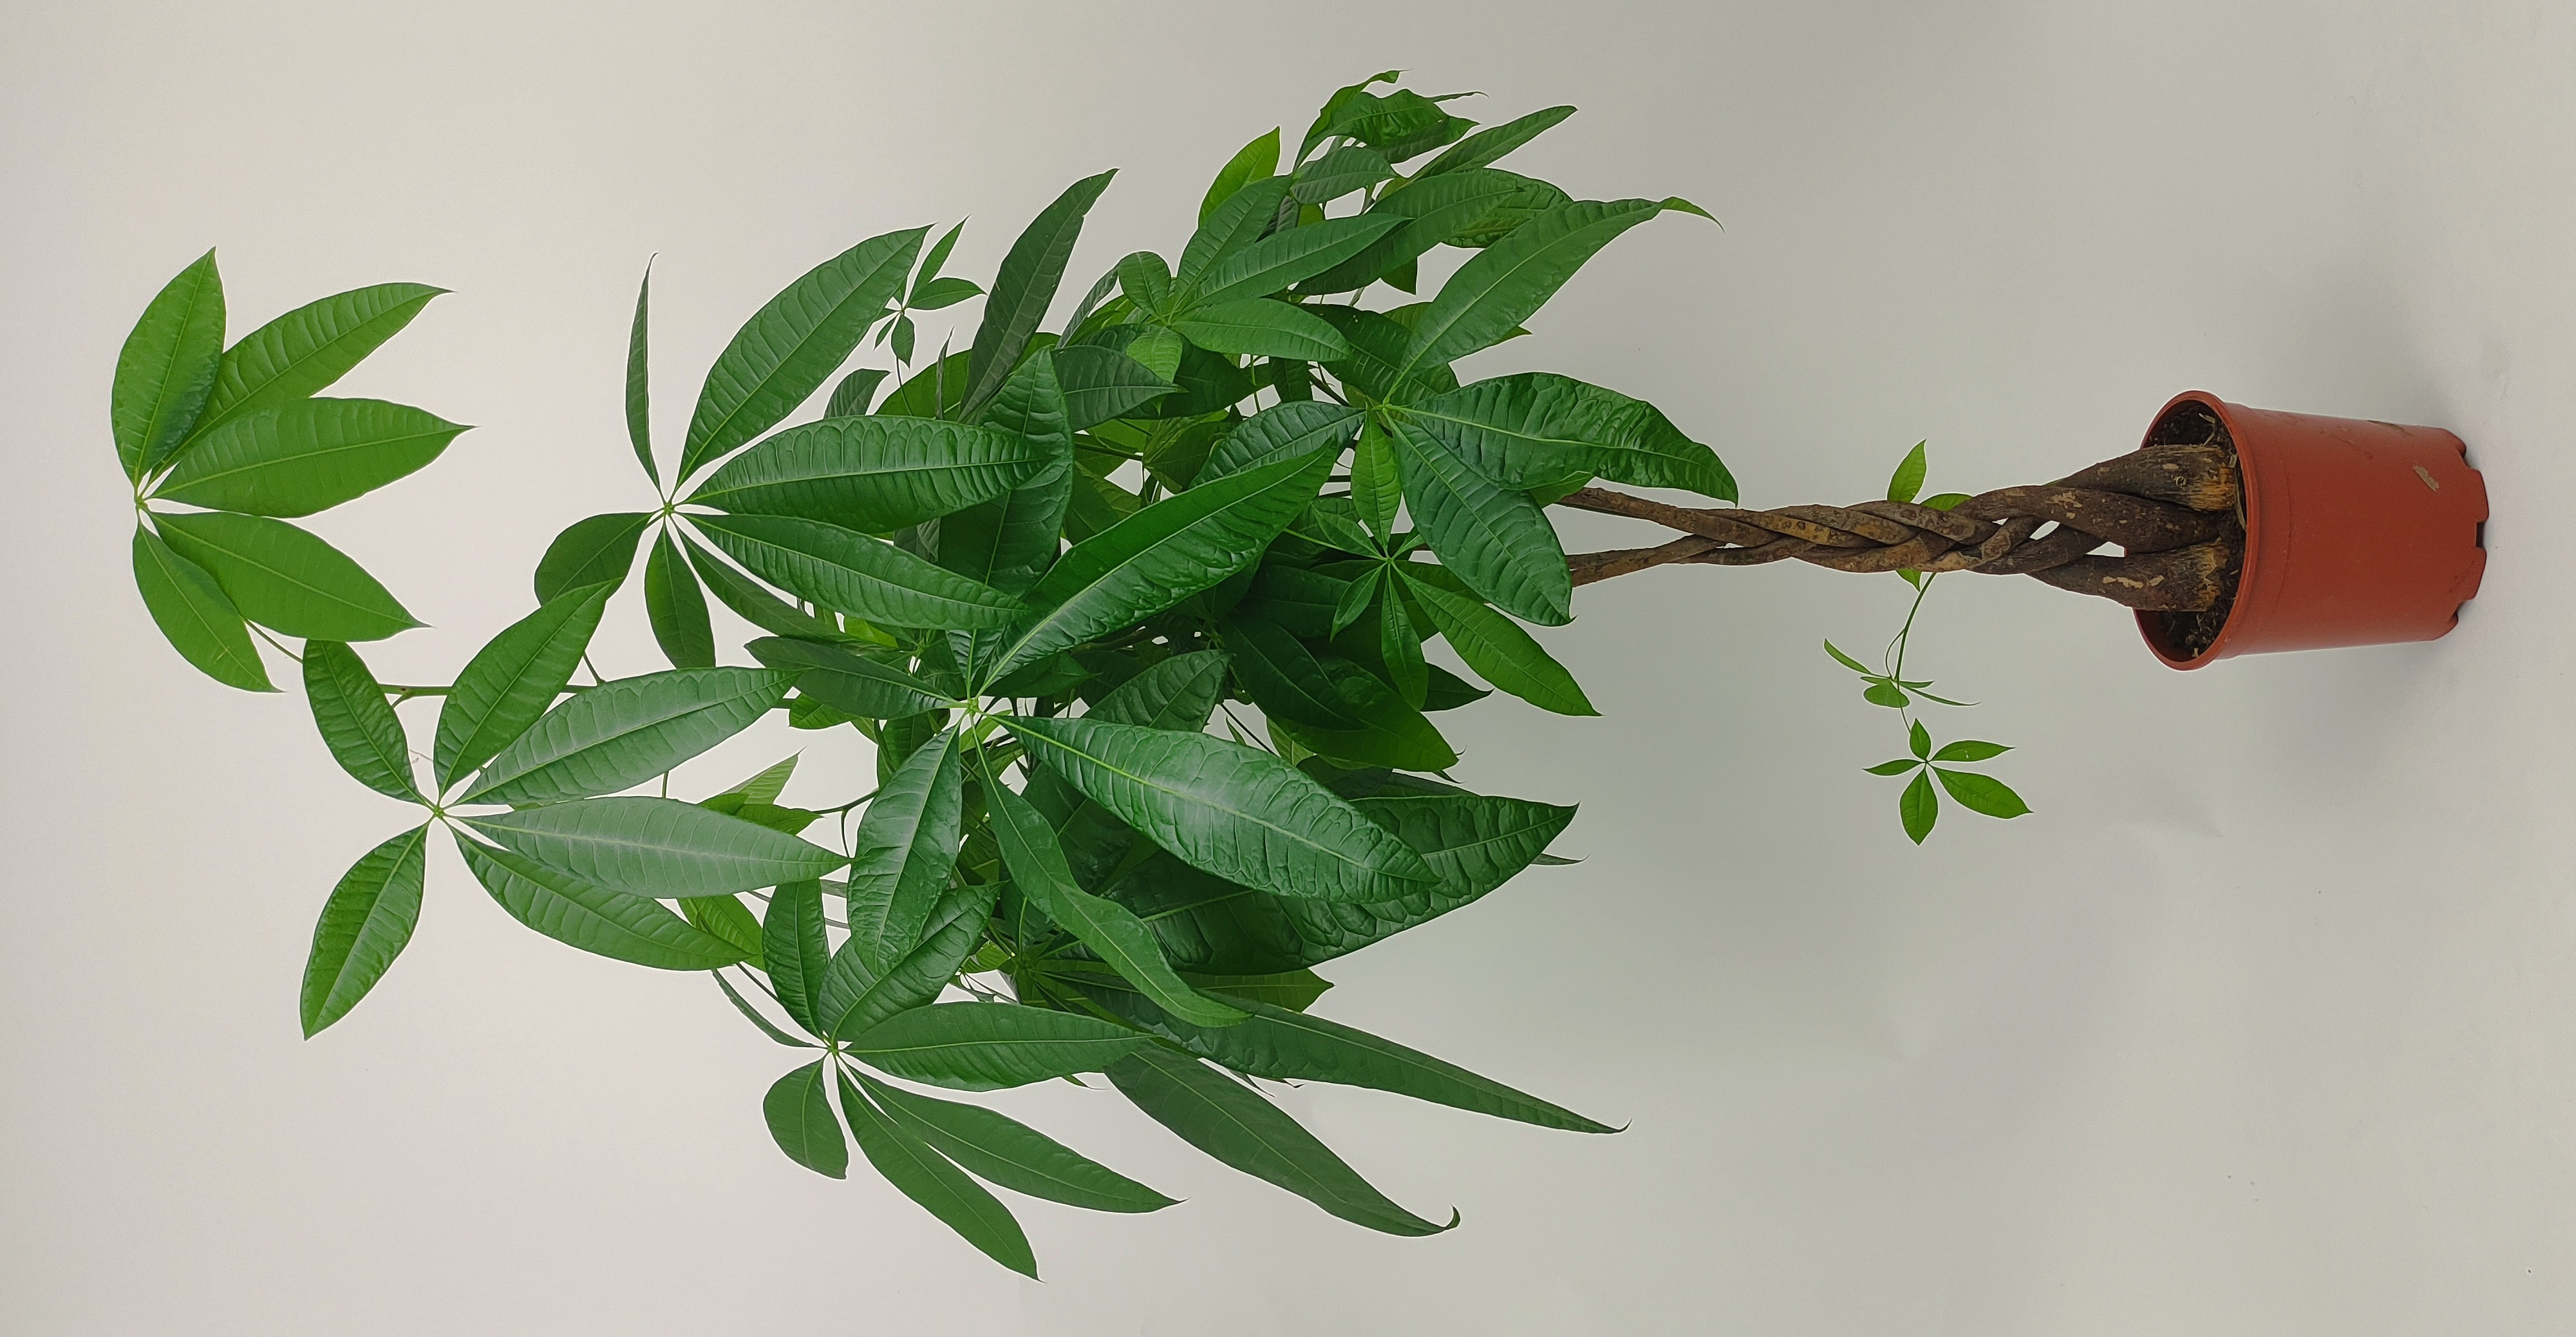
\includegraphics[width=0.42\textwidth, angle=-90]{Images/tall_plant_cropped.jpg}
    \caption{The plant N°2 is a \textit{Pachira glabra}.}
    
    \vspace{-0.5cm}
    \label{fig:tall_plant}
    \vspace{0.2cm}
\end{figure}


\newpage

\subsubsection{Dypsis lutescens}

The \textit{Dypsis lutescens} is composed of many trunks and stems. On top of that, the leaves are numerous and tight. The plant is 100cm tall.

\begin{figure}[ht]
    \centering
    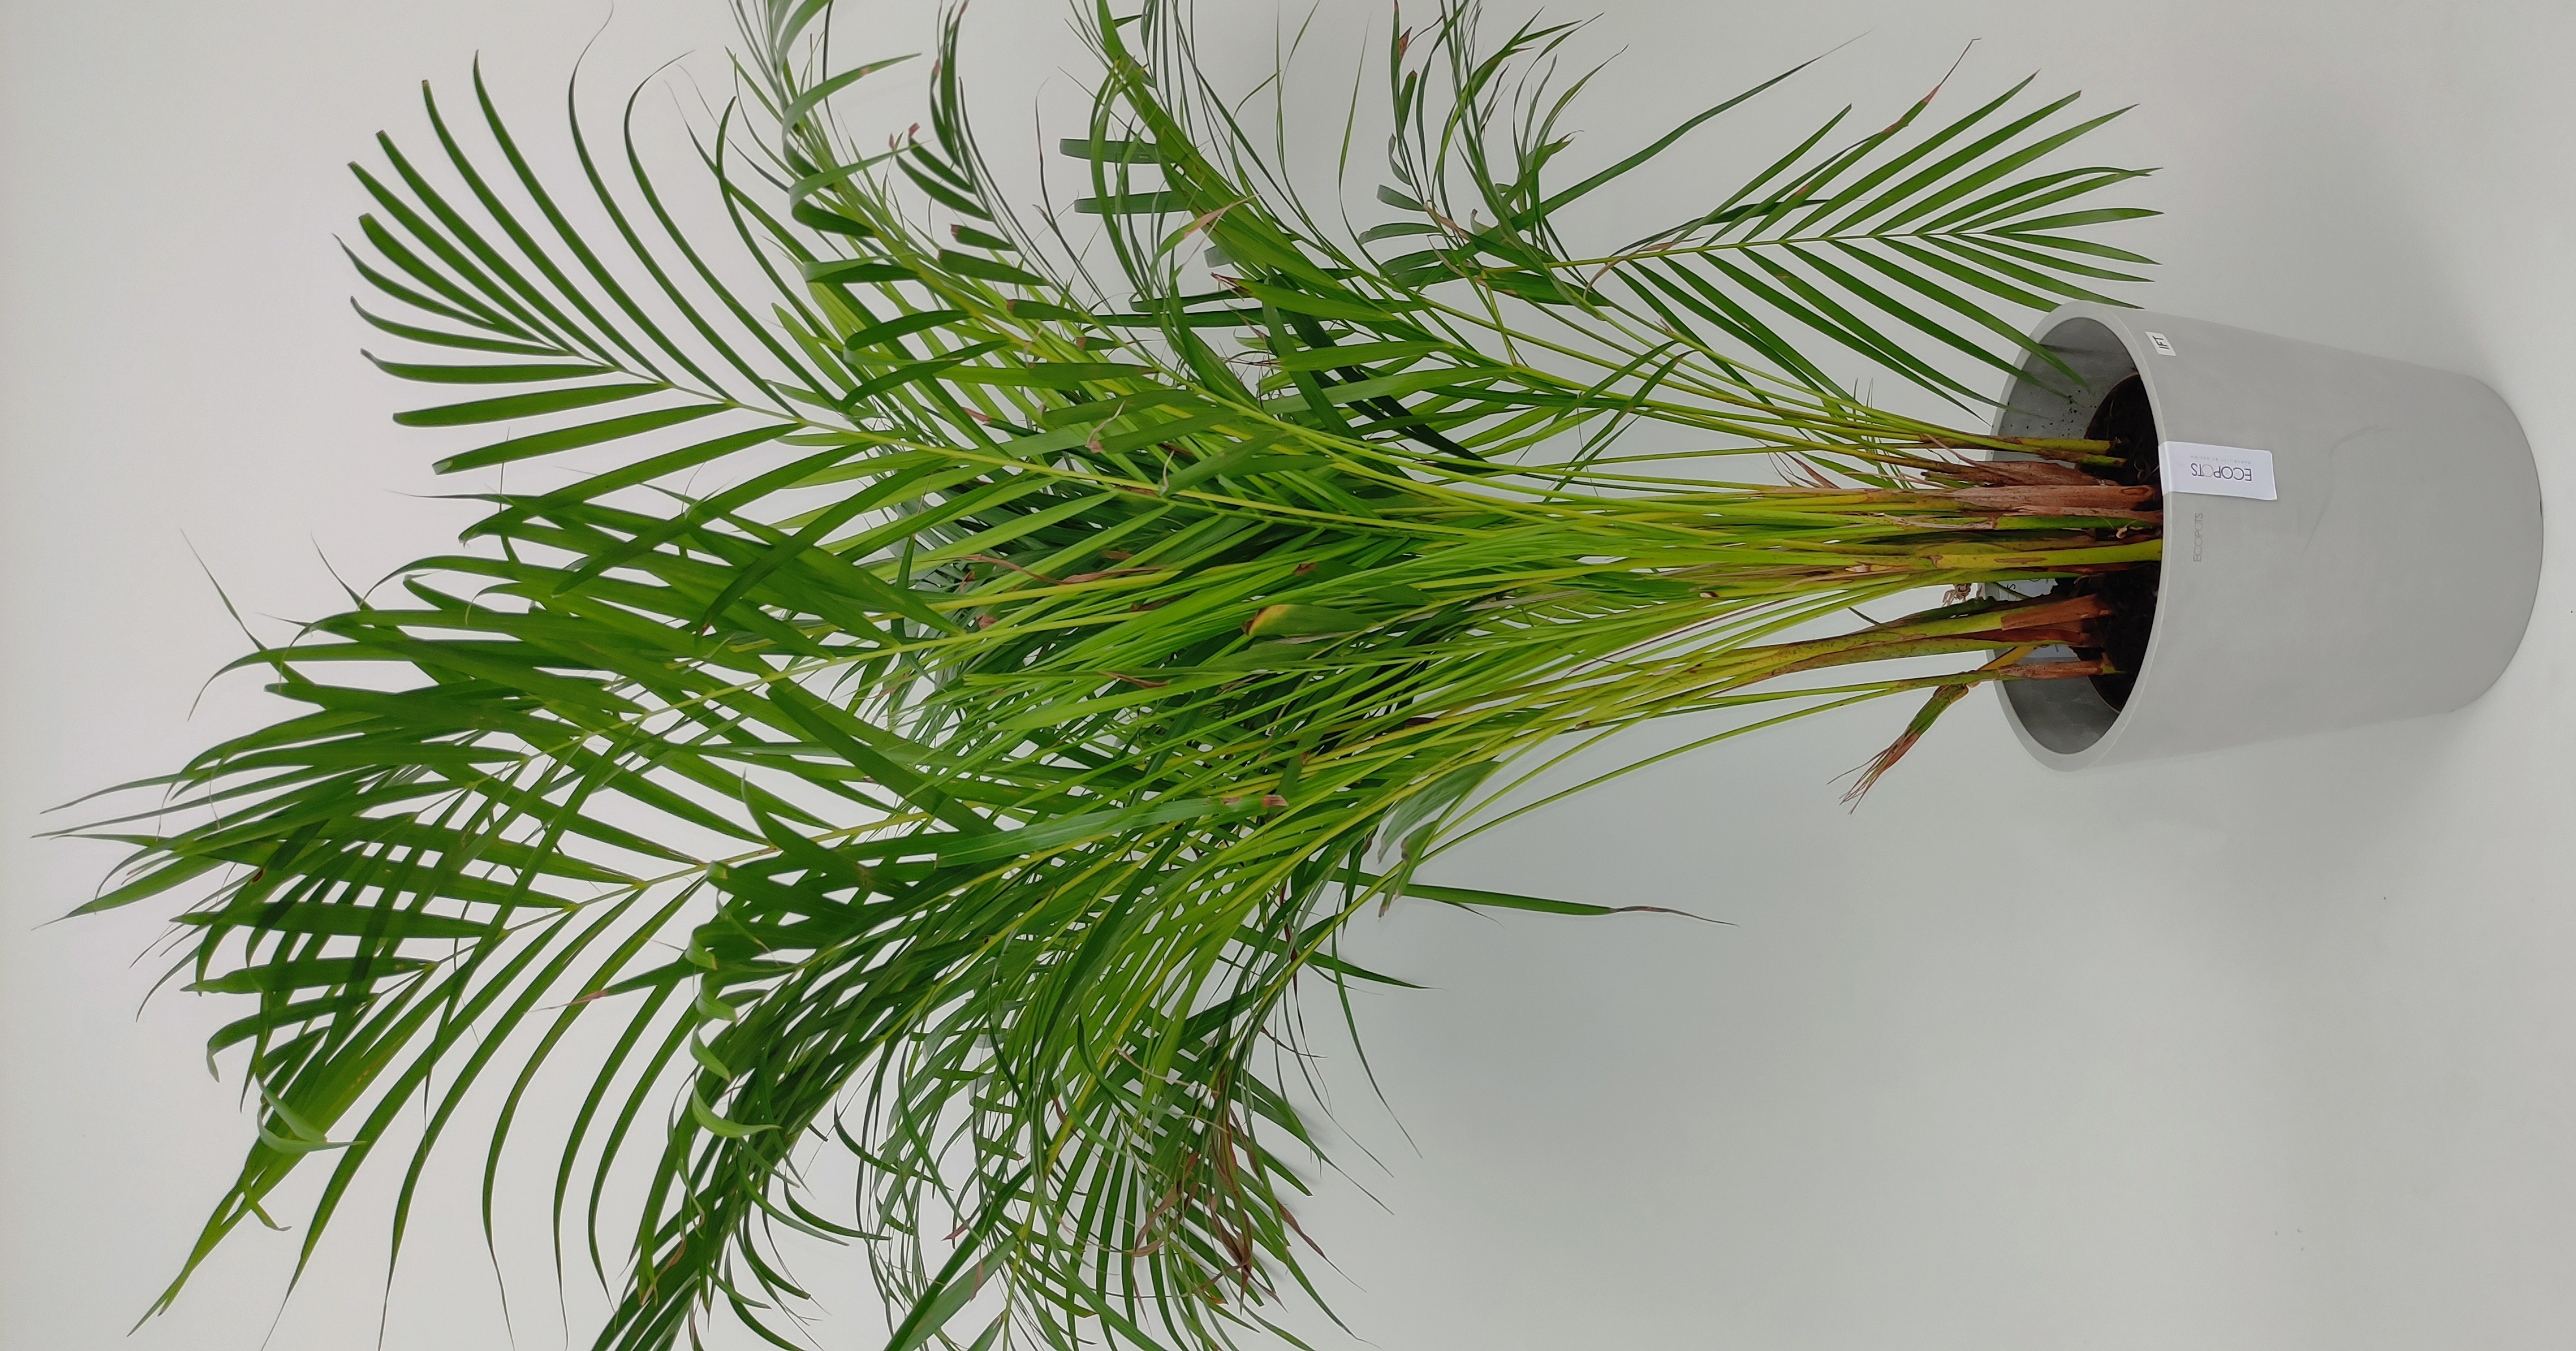
\includegraphics[width=0.42\textwidth, angle=-90]{Images/fougere_plant.jpg}
    \caption{The plant N°3 is a \textit{Dypsis lutescens}.}
    
    \vspace{-0.5cm}
    \label{fig:fougere_plant}
    \vspace{0.2cm}
\end{figure}



\subsubsection{The experimental space}

The experimental space featured three distinct levels of height, each corresponding to one of the three plants introduced to participants.

\begin{figure}[h]
    \centering
    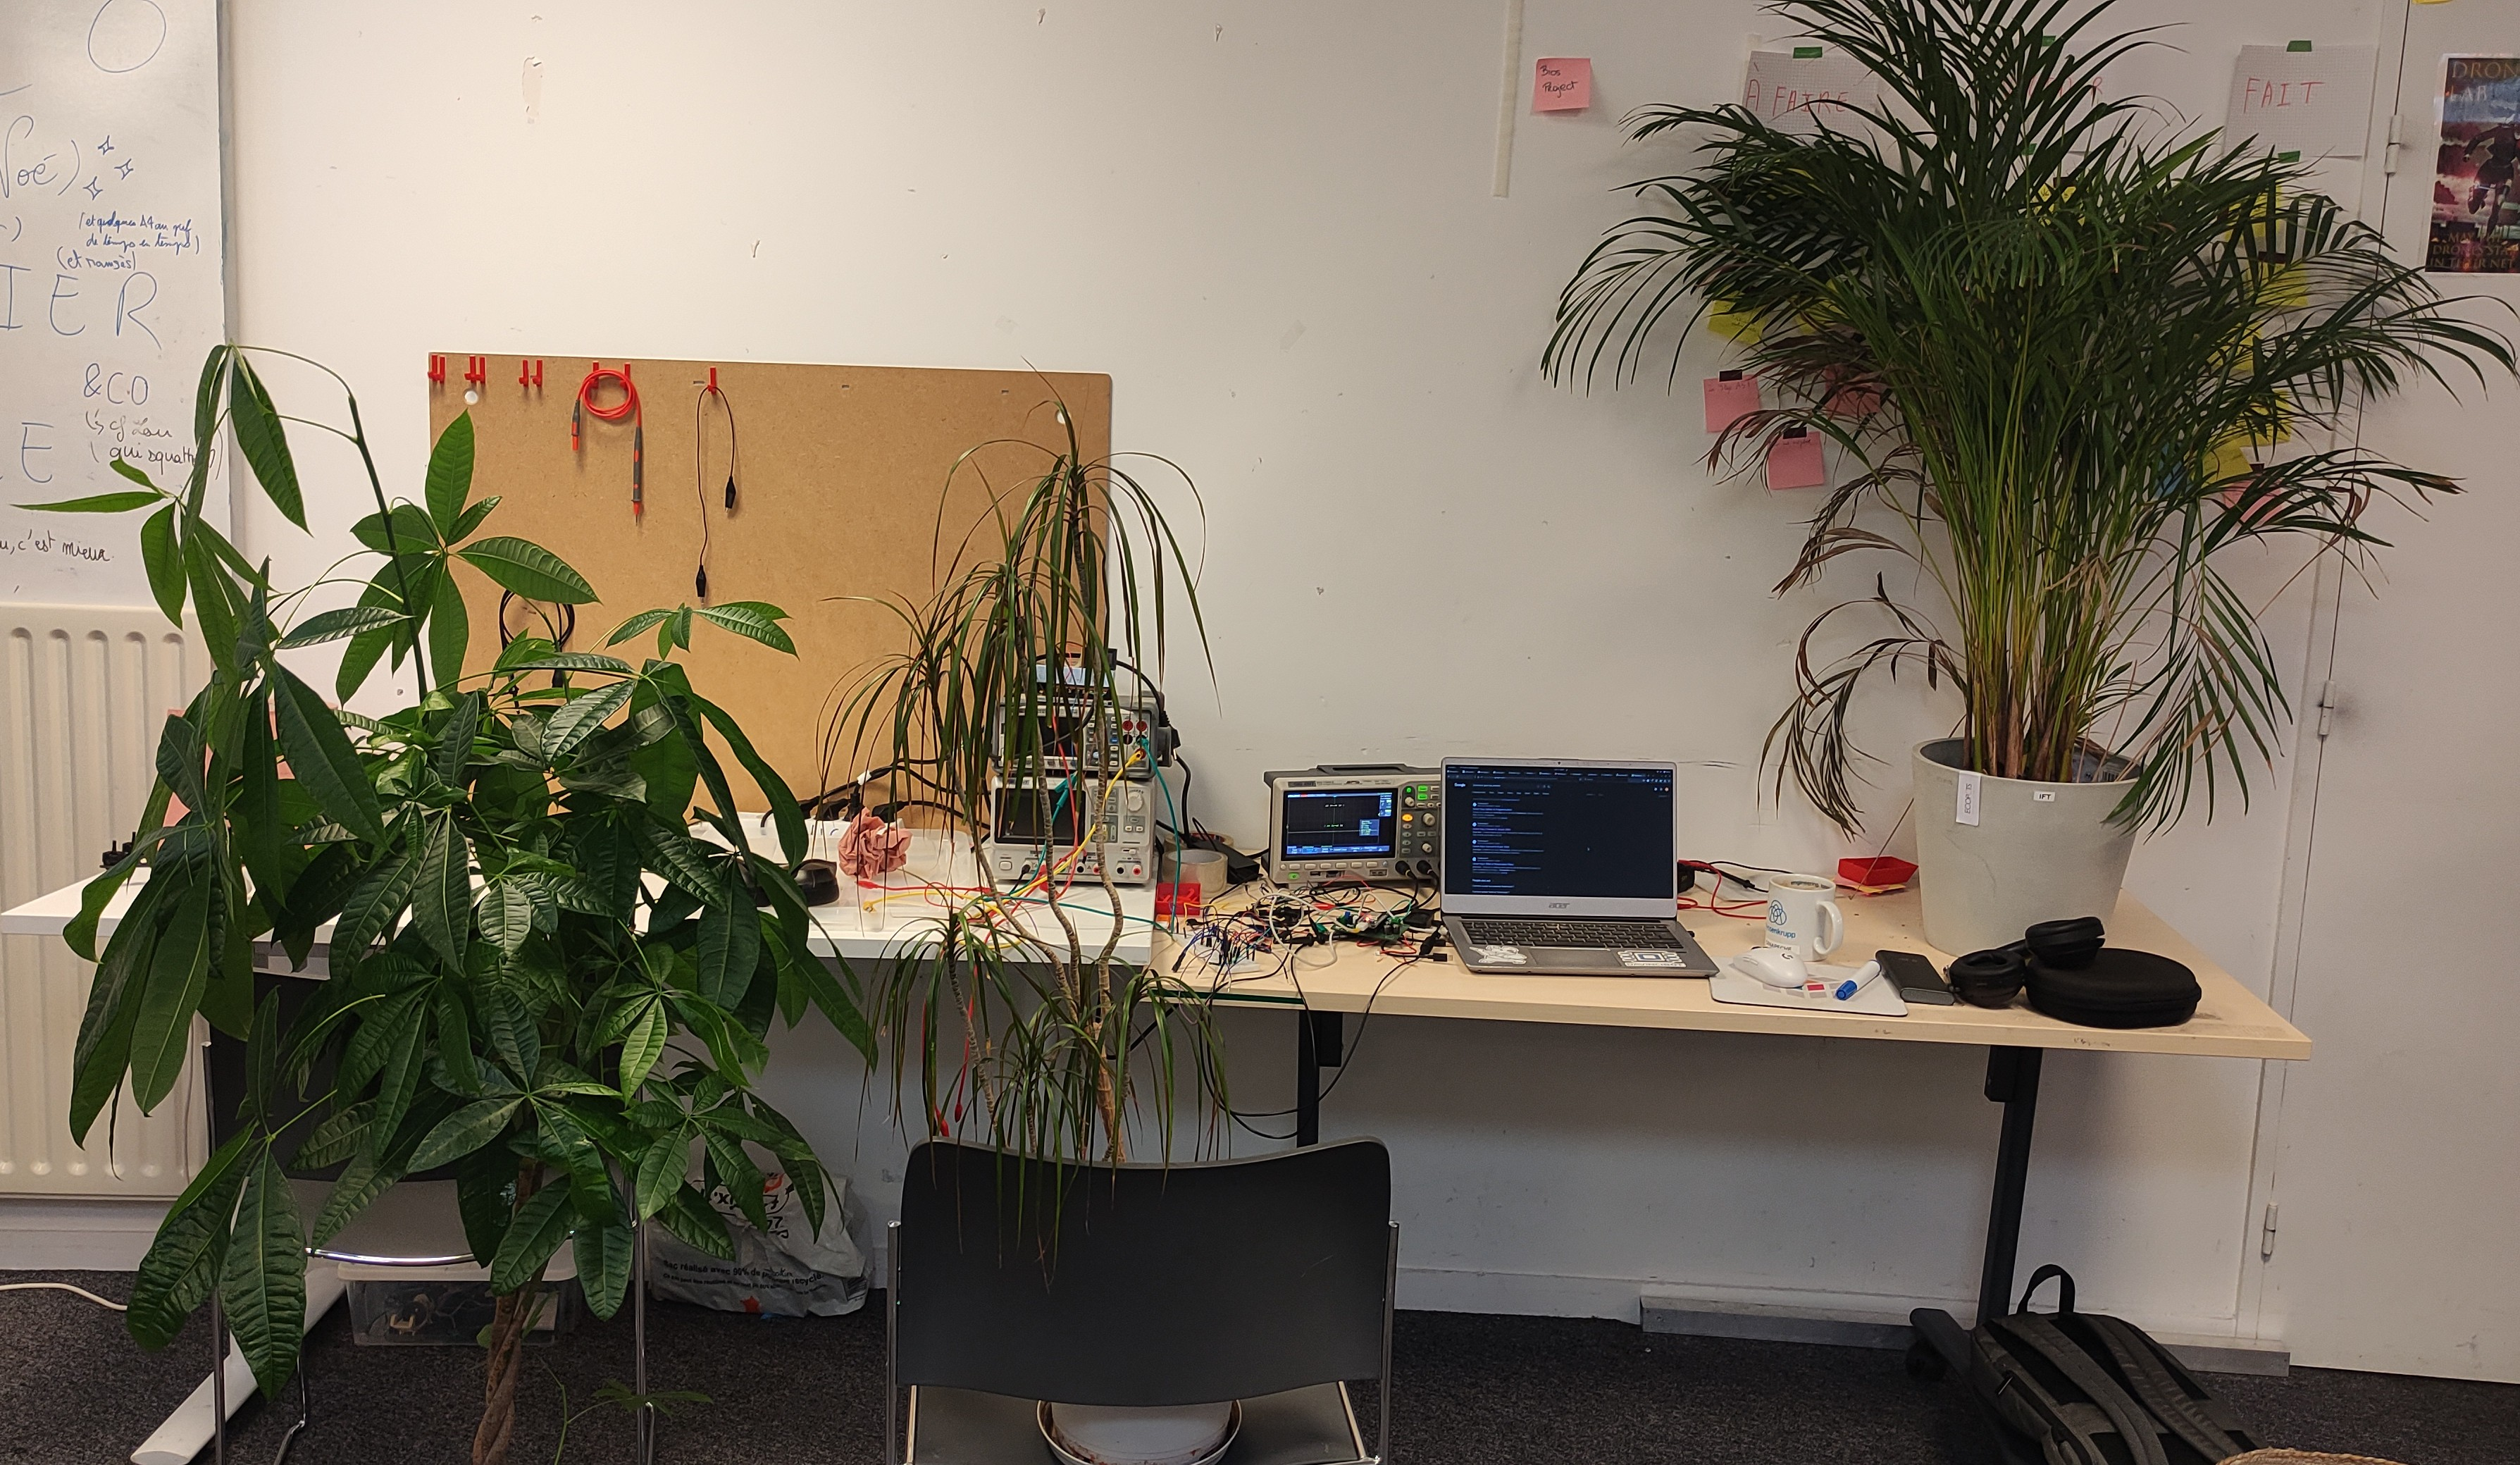
\includegraphics[width=0.42\textwidth]{Images/setup_user_study.jpg}
    \caption{User study space setup. The set-up is built from our lab space.}
    
    \vspace{-0.5cm}
    \label{fig:setup_user_study}
    \vspace{0.2cm}
\end{figure}

\newpage

